%
% -----------------------------------------------------------------------------
\section{Model description}
The model used for this demo corresponds to the model proposed by 
\citet{midzi1999} in the context of the GSHAP project.
As illustrated in Figure \ref{fig:ssa_area_sources}, this 
seismic source model contains 21 area sources distributed along a wide 
band ideally connecting from the Red Sea with South Africa.

The area sources part of this model can be ideally subdivided into a small 
number of groups.
To the north, a first class of area sources cover the three branches 
of the triple junction in the Afar region. 
The following set of sources shows a spatial pattern that reproduces
the structural trend of the graben systems composing the two main 
branches composing the continental part of the East African Rift:
the Western and East branches. The last set of sources includes the 
southermost part of the model where rift's textonic structure are less
evident and the seismicity spreads over a wide sectors (see Figure
\ref{fig:Subsahara_Catalogue_ISC_1}).
%
\begin{figure}[ht]
	\centering
	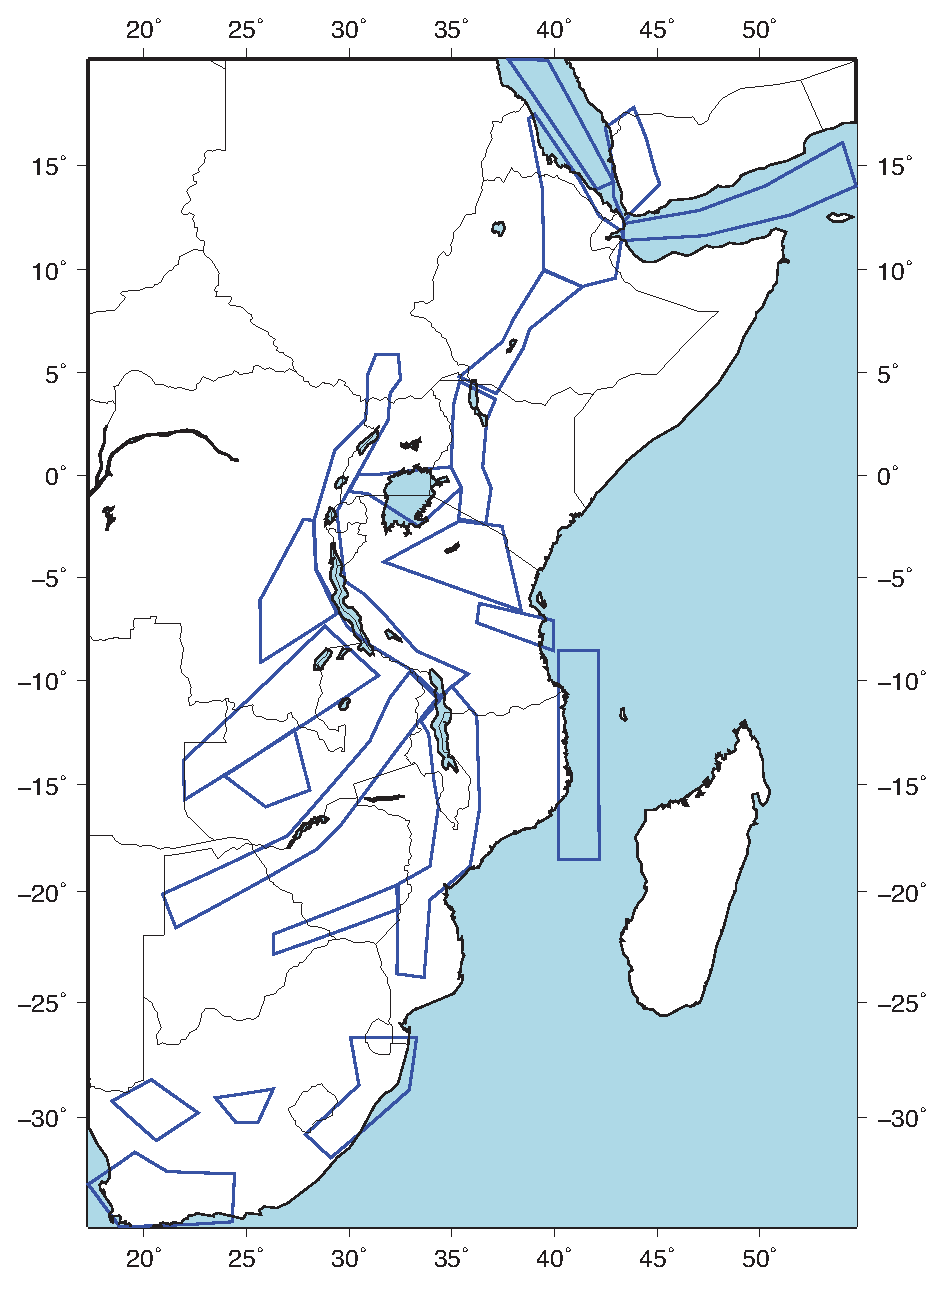
\includegraphics[width=10cm]
        {./figures/ssa_area_sources.eps}
	\caption{Area sources in the demo PSHA input model.}
	\label{fig:ssa_area_sources}
\end{figure}
%
The seismicity recurrence parameters and the maximum magnitude 
assigned to the different sources corresponds to the ones originally
determined by \citet{midzi1999}.

The maximum magnitude ranges between 6.5 and 7.8; the sources with the
highest potential 

The 

%
% -----------------------------------------------------------------------------
\section{Assignment: hazard calculation using the demo model}
The first assignment focuses on the calculation of hazard for a small area 
using Openquake and demo model provided.


\clearpage
%
% -----------------------------------------------------------------------------
\subsection{Analysis of results}
